\documentclass[10pt, aspectratio=169]{beamer}

% Theme and styling setup
\usetheme{Madrid}
\usecolortheme{whale}

% Font and language configuration
\usepackage{fontspec}
\usepackage[german]{babel}
\usepackage{amsmath}
\usepackage{booktabs}
\usepackage{graphicx}
\usepackage{tikz}
\usetikzlibrary{positioning, arrows.meta}

% Color definitions
\definecolor{maincolor}{RGB}{30, 58, 138}    % Deep Navy Blue
\definecolor{accentcolor}{RGB}{13, 148, 136}  % Teal Accent
\definecolor{bglight}{RGB}{248, 250, 252}     % Slate Light Gray
\definecolor{alertred}{RGB}{220, 38, 38}      % Alert Red

\setbeamercolor{palette primary}{bg=maincolor, fg=white}
\setbeamercolor{palette secondary}{bg=accentcolor, fg=white}
\setbeamercolor{structure}{fg=maincolor}
\setbeamercolor{frametitle}{bg=maincolor, fg=white}
\setbeamercolor{block title}{bg=maincolor, fg=white}
\setbeamercolor{block body}{bg=bglight, fg=black}

\title[Phishing \& Social Engineering]{Phishing, Social Engineering \& Best Practices}
\subtitle{Informatik | Kantonsschule im Lee}
\author{Laurin Ott}
\date{23. November 2026}

\begin{document}

% -----------------------------------------------------------------------------
% TITLE SLIDE
% -----------------------------------------------------------------------------
\begin{frame}
  \titlepage
\end{frame}

% -----------------------------------------------------------------------------
% EINSTIEG & GRUNDLAGEN
% -----------------------------------------------------------------------------
\begin{frame}{Echt oder Phishing?}
  \pause
  \begin{block}{Echt oder Phishing?}
    Wir starten direkt mit einem interaktiven Test, nämlich mit dem \textbf{Google Phishing Quiz} (\texttt{phishingquiz.withgoogle.com}).
  \end{block}
  \vspace{0.8em}
  \pause
  \begin{block}{So läuft es ab}
    \begin{enumerate}
      \item Öffnen Sie den Link auf Ihren Geräten (Moodle).
      \item Lösen Sie die 10 Fragen.
      \item Notieren Sie sich die Ergebnisse für die anschliessende Diskussion.
    \end{enumerate}
  \end{block}
\end{frame}

% -----------------------------------------------------------------------------
% SOCIAL ENGINEERING & KLASSISCHES VS. SPEAR-PHISHING
% -----------------------------------------------------------------------------
\begin{frame}{Social Engineering}
  \pause
  \begin{block}{Was ist Social Engineering?}
    Statt komplexe technische Systeme direkt zu hacken, manipulieren Angreifer gezielt die \textbf{menschliche Psyche}, um an vertrauliche Daten zu gelangen oder Schadsoftware zu verbreiten.
  \end{block}

  \vspace{0.6em}
  \begin{columns}[T]
    \pause
    \begin{column}{0.48\textwidth}
      \begin{block}{Klassisches Phishing}
        \begin{itemize}
          \item Richtet sich ungezielt an eine \textbf{breite Masse}.
          \item Täuschend echte Massen-E-Mails im Namen bekannter Banken, Streaming-Dienste oder Behörden.
        \end{itemize}
      \end{block}
    \end{column}

    \pause
    \begin{column}{0.48\textwidth}
      \begin{block}{Spear-Phishing}
        \begin{itemize}
          \item \textbf{Hochspezifischer, massgeschneiderter Angriff} auf eine einzelne Person oder bestimmte Mitarbeitende.
          \item Nutzt persönliche Informationen, um gezielt Vertrauen zu erwecken.
        \end{itemize}
      \end{block}
    \end{column}
  \end{columns}
\end{frame}

% -----------------------------------------------------------------------------
% WEITERE ANGRIFFSKANÄLE
% -----------------------------------------------------------------------------
\begin{frame}{Angriffskanäle im Überblick}
  \pause
  \begin{columns}[T]
    \begin{column}{0.31\textwidth}
      \begin{block}{Vishing (Voice)}
        \small
        \begin{itemize}
          \item Betrugsversuche über \textbf{Telefonanrufe}.
          \item Anrufer gibt sich als vertrauenswürdige Stelle aus.
          \item Ziel: Passwörter, PINs oder TANs abfragen.
        \end{itemize}
      \end{block}
    \end{column}

    \pause
    \begin{column}{0.31\textwidth}
      \begin{block}{Smishing (SMS)}
        \small
        \begin{itemize}
          \item Betrug über \textbf{Kurznachrichten (SMS)}.
          \item Warnung vor angeblicher Kontosperrung oder Paketproblemen.
          \item Lockt auf schädliche Kurzlinks.
        \end{itemize}
      \end{block}
    \end{column}

    \pause
    \begin{column}{0.31\textwidth}
      \begin{block}{Quishing (QR-Code)}
        \small
        \begin{itemize}
          \item Platzieren manipulierter \textbf{QR-Codes} (z.\,B. auf Plakaten oder Parkuhren).
          \item Leitet unbemerkt auf gefälschte Webseiten weiter.
        \end{itemize}
      \end{block}
    \end{column}
  \end{columns}
  \pause
  \vspace{1em}
  \centering
  \textit{Merke: Phishing findet längst nicht mehr nur im klassischen E-Mail-Postfach statt!}
\end{frame}

% -----------------------------------------------------------------------------
% PSYCHOLOGISCHE FAKTOREN
% -----------------------------------------------------------------------------
\begin{frame}{Psychologische Faktoren und Wirkungsweise}
  \pause
  \textbf{Warum fallen Menschen auf Phishing herein?} Angreifer nutzen gezielt emotionale Hebel aus, um kritisches Denken auszuschalten:
  \vspace{0.8em}

  \begin{columns}[T]
    \pause
    \begin{column}{0.48\textwidth}
      \begin{alertblock}{1. Angst \& Drohungen}
        Drohende Konsequenzen wie \textbf{angebliche Kontosperrungen} oder unbezahlte Rechnungen erzeugen Panik.
      \end{alertblock}
      \vspace{0.5em}
      \pause
      \begin{alertblock}{2. Zeitdruck / Dringlichkeit}
        Kurze Fristen (\textit{«innerhalb von 120 Minuten»}) verleiten dazu, übereilt und unüberlegt zu handeln.
      \end{alertblock}
    \end{column}

    \pause
    \begin{column}{0.48\textwidth}
      \begin{block}{3. Neugier \& Gier}
        Versprechen von \textbf{verpassten Gewinnen}, Rückerstattungen oder exklusiven Informationen locken zum Klick.
      \end{block}
      \vspace{0.5em}
      \pause
      \begin{block}{4. Hilfsbereitschaft}
        Vermeintliche Anfragen von Vorgesetzten oder Bekannten nutzen Vertrauen und Autoritätsglauben aus.
      \end{block}
    \end{column}
  \end{columns}
\end{frame}

% -----------------------------------------------------------------------------
% EINZELARBEIT & SICHERUNG
% -----------------------------------------------------------------------------
\begin{frame}{Arbeitsphase 1}
  \pause
  \begin{block}{Zu zweit im Skript}
    Bearbeiten Sie zu zweit im Skript:
    \begin{itemize}
      \item \textbf{Aufgabe 7:} Klassisches Phishing vs. Spear-Phishing
      \item \textbf{Aufgabe 8:} Gefahrenkanäle (Vishing, Smishing \& Quishing) zuordnen
      \item \textbf{Aufgabe 10:} Drei psychologische Tricks und deren Wirkung beschreiben
    \end{itemize}
  \end{block}
\end{frame}

% -----------------------------------------------------------------------------
% ENTWICKLUNG EINES EIGENEN PHISHING-BEISPIELS
% -----------------------------------------------------------------------------
\begin{frame}{Eigenes Phishing-Beispiel entwickeln}
  \pause
  \begin{exampleblock}{Auftrag in 2er-Teams}
    Entwerfen Sie ein möglichst überzeugendes \textbf{Spear-Phishing- oder Smishing-Beispiel} für ein fiktives Szenario (z.\,B. \textit{Kanti-IT-Support, TWINT-Rückerstattung, SBB-Halbtax, Galaxus-Paket}).
  \end{exampleblock}

  \vspace{0.6em}
  \pause
  \begin{block}{Checkliste für euren Entwurf}
    \begin{itemize}
      \item \textbf{Psychologie:} Mindestens 2 Trigger einbauen (z.\,B. Angst + Zeitdruck).
      \item \textbf{Technik:} Täuschenden Absender und eine manipulierte URL (\textbf{Typosquatting}) erfinden.
      \item \textbf{Wichtig:} Nur lokal als Text/Entwurf erstellen, niemals echte Links verwenden oder versenden!
    \end{itemize}
  \end{block}
\end{frame}

% -----------------------------------------------------------------------------
% BEST PRACTICES
% -----------------------------------------------------------------------------
\begin{frame}{Aktuelle Richtlinien \& Best Practices}
  \pause
  \begin{columns}[T]
    \begin{column}{0.55\textwidth}
      \begin{block}{Die wichtigsten Schutzregeln}
        \small
        \begin{enumerate}
          \pause
          \item \textbf{Kritische Hürden bewahren:} Nie unüberlegt auf Links klicken oder Anhänge öffnen.
          \pause
          \item \textbf{Absender \& URLs prüfen:} Auf Buchstabendreher (\textbf{Typosquatting}) achten.
          \pause
          \item \textbf{Keine sensiblen Daten:} Banken fragen nie per Mail/SMS/Telefon nach Passwörtern.
          \pause
          \item \textbf{Druck hinterfragen:} Drohungen und kurze Fristen kritisch prüfen.
          \pause
          \item \textbf{Direktzugriff bevorzugen:} Webseiten immer manuell im Browser aufrufen.
        \end{enumerate}
      \end{block}
    \end{column}

    \pause
    \begin{column}{0.42\textwidth}
      \begin{alertblock}{Achtung: Moderne KI-Tools}
        \small
        Unpersönliche Anreden und Grammatikfehler bleiben wichtige Warnsignale.
        \vspace{0.6em}

        \textbf{Aber:} Durch generative KI erstellen Angreifer heute sprachlich einwandfreie Texte. \textbf{Fehlerfreiheit ist kein Garantiebeweis für Echtheit!}
      \end{alertblock}
    \end{column}
  \end{columns}
\end{frame}

% -----------------------------------------------------------------------------
% VORSTELLUNG DER BEISPIELE
% -----------------------------------------------------------------------------
\begin{frame}{Showdown der Phishing-Beispiele}
  \pause
  \begin{block}{Vorstellung \& Analyse im Plenum}
    \begin{enumerate}
      \item Jedes 2er-Team zeigt kurz sein erstelltes Phishing-Beispiel aus Lektion 1.
      \item Die anderen Teams agieren als Security-Analysten: \textbf{Welche «Red Flags» und psychologischen Tricks wurden eingebaut?}
    \end{enumerate}
  \end{block}
\end{frame}

% -----------------------------------------------------------------------------
% MFA & LIVE-PHISHING
% -----------------------------------------------------------------------------
\begin{frame}{Live-Phishing}
  \pause
  \begin{block}{Warum MFA schützt und wann sie versagt}
    \textbf{Standard-MFA} erschwert Kontoübernahmen massiv, da ein abgefangenes Passwort ohne den zweiten Faktor nutzlos ist. Beim \textbf{Live-Phishing} schalten Angreifer jedoch einen Proxy in Echtzeit dazwischen:
  \end{block}

  \vspace{0.6em}
  \pause
  \centering
  \begin{tikzpicture}[
      font=\sffamily\small,
      >=Latex,
      box/.style={rectangle, draw=maincolor, thick, rounded corners=4pt, fill=bglight, minimum width=3.2cm, minimum height=1.3cm, align=center},
      evil/.style={rectangle, draw=alertred, very thick, rounded corners=4pt, fill=red!5, minimum width=3.6cm, minimum height=1.3cm, align=center}
  ]
    \node[box] (victim) {\textbf{1. Opfer}\\Gibt Passwort \&\\Einmalcode ein};
    \node[evil, right=1.6cm of victim] (proxy) {\textcolor{alertred}{\textbf{2. Phishing-Proxy}}\\Fängt Passwort \& MFA\\in Echtzeit ab};
    \node[box, right=1.6cm of proxy] (real) {\textbf{3. Echte Website}\\Angreifer loggt sich\\sofort gültig ein};

    \draw[->, very thick, alertred] (victim) -- node[above, font=\scriptsize] {Live-Daten} (proxy);
    \draw[->, very thick, alertred] (proxy) -- node[above, font=\scriptsize] {Weiterleitung} (real);
  \end{tikzpicture}

  \pause
  \vspace{0.8em}
  \textit{Fazit: Auch bei aktiver MFA gilt. Immer zuerst die URL prüfen und Direktzugriffe nutzen!}
\end{frame}

% -----------------------------------------------------------------------------
% PARTNERARBEIT & BESPRECHUNG
% -----------------------------------------------------------------------------
\begin{frame}{Arbeitsphase 2}
  \pause
  \begin{block}{Partnerarbeit im Skript}
    Lösen Sie zu zweit im Skript:
    \begin{itemize}
      \item \textbf{Aufgabe 9:} Schutzwirkung von MFA bei Phishing erklären
      \item \textbf{Aufgabe 11:} Szenario-Analyse der Bank-Mail
      \item \textbf{Aufgabe 12:} Sicherheitsrichtlinien beurteilen
    \end{itemize}
  \end{block}
\end{frame}

% -----------------------------------------------------------------------------
% FEEDBACK & ZUSATZ
% -----------------------------------------------------------------------------
\begin{frame}{Unterrichts-Feedback \& Abschluss}
  \pause
  \begin{center}
    \Large \textbf{Vielen Dank für Ihre aktive Mitarbeit!}

    \pause
    \vspace{1.5em}
    
\includegraphics[width=0.3\textwidth]{qrcode_Quishing.png}
  \end{center}
\end{frame}

\begin{frame}{Unterrichts-Feedback \& Abschluss}
  \pause
  \begin{center}
    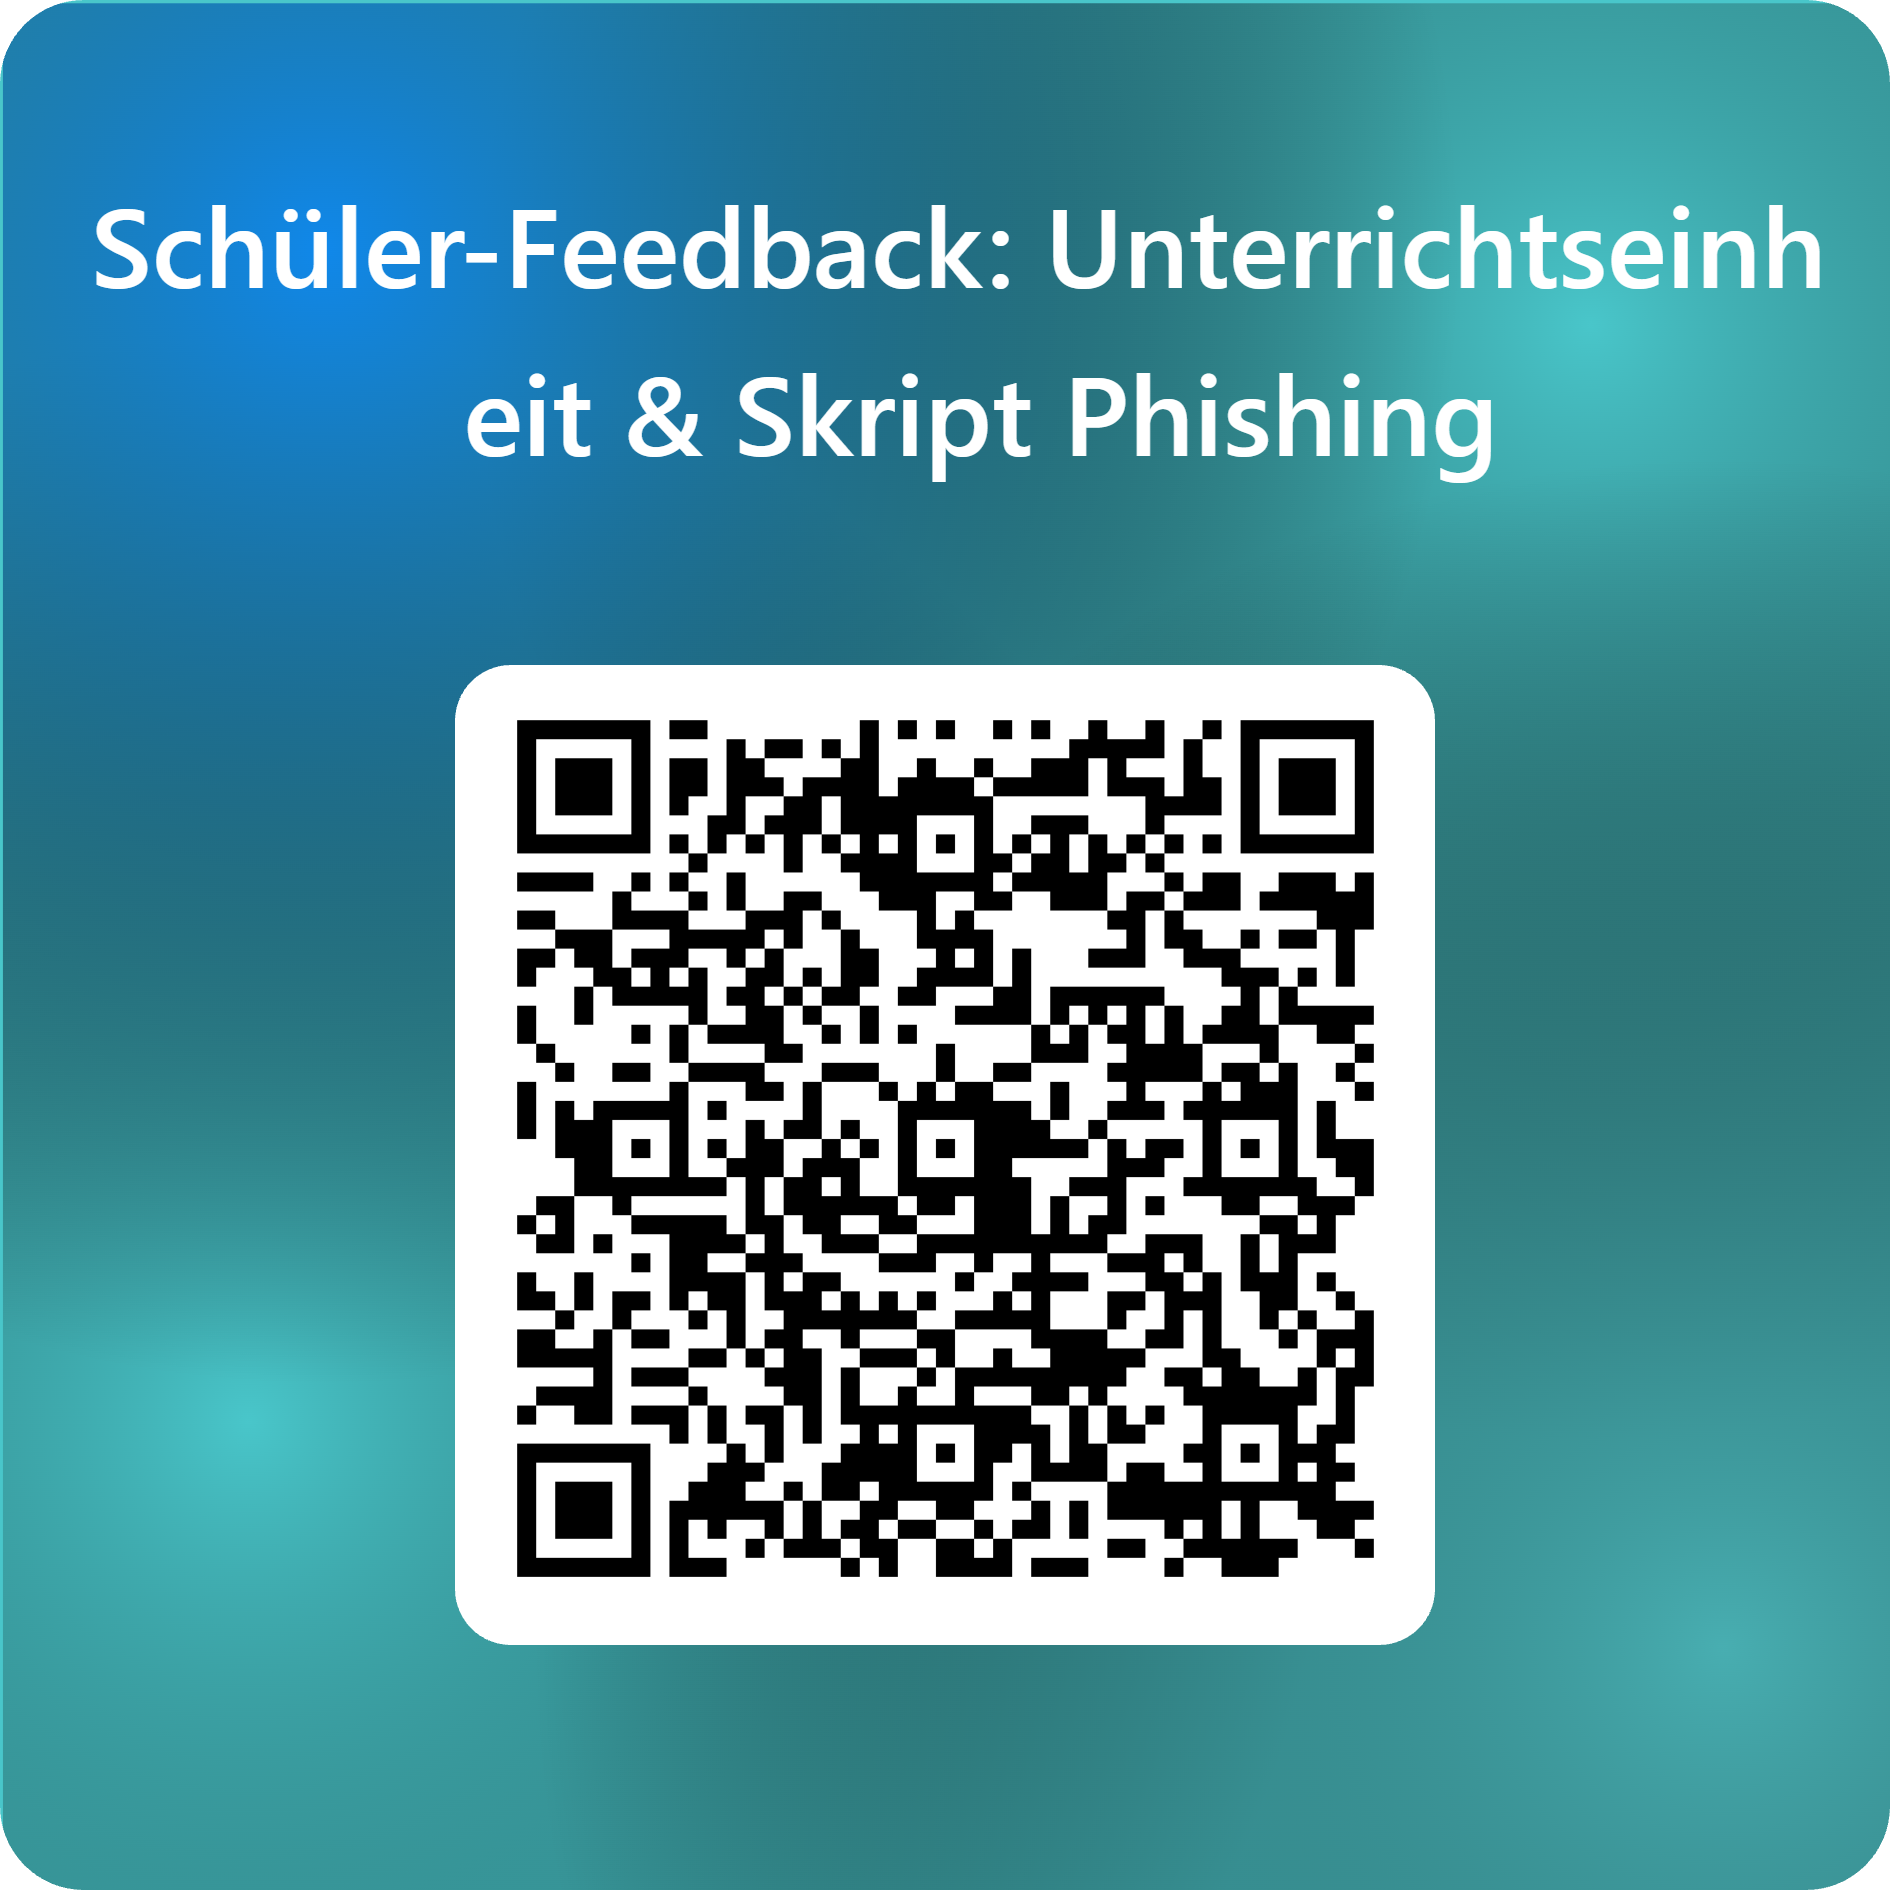
\includegraphics[width=0.4\textwidth]{QRCode für Feedback Phishing.png}
  \end{center}
\end{frame}

\begin{frame}{Zusatz: Wurden eure Daten schon geleakt?}
  \pause
  \begin{block}{Praxis-Check: \texttt{haveibeenpwned.com}}
    \begin{itemize}
      \item Öffnen Sie \texttt{haveibeenpwned.com} im Browser.
      \item Prüfen Sie (freiwillig) mit Ihrer E-Mail-Adresse, ob Ihre Daten bereits in einem bekannten \textbf{Datenleck} aufgetaucht sind.
      \item Schauen Sie nach, welche Plattformen betroffen waren und welche Daten (E-Mail, Passwort, Telefonnummer) abgeflossen sind, genau solche Datensätze nutzen Angreifer für gezieltes \textbf{Spear-Phishing}!
    \end{itemize}
  \end{block}
\end{frame}

% -----------------------------------------------------------------------------
% ANHANG: VERLAUFSPLANUNG FÜR LEHRPERSONEN (HALBKLASSE)
% -----------------------------------------------------------------------------
\appendix
\begin{frame}{Anhang: Verlaufsplanung für Lehrpersonen (10 SuS)}
  \begin{columns}[T]
    \begin{column}{0.48\textwidth}
      \begin{block}{Lektion 1: Grundlagen \& Psychologie (45 Min.)}
        \small
        \begin{itemize}
          \item \textbf{00--15 min:} Einstieg
          \item \textbf{15--30 min:} Einzelarbeit Aufgaben 7, 8 \& 10
          \item \textbf{30--35 min:} Sicherung \& Abgleich im Plenum
          \item \textbf{35--45 min:} Entwicklung eines eigenen Phishing-Beispiels
        \end{itemize}
      \end{block}
    \end{column}
    \begin{column}{0.48\textwidth}
      \begin{block}{Lektion 2: Abwehr \& Transfer (45 Min.)}
        \small
        \begin{itemize}
          \item \textbf{00--05 min:} Best Practices
          \item \textbf{05--15 min:} Phishing-Beispiel aus Lektion 1 vorstellen 
          \item \textbf{15--20 min:} Live-Phishing \& MFA
          \item \textbf{20--30 min:} Partnerarbeit Aufgaben 9, 11 \& 12
          \item \textbf{30--40 min:} Besprechung im Plenum 
          \item \textbf{40--45 min:} Feedback
          \item \textbf{Zusatz:} Have I been pwned?
        \end{itemize}
      \end{block}
    \end{column}
  \end{columns}
\end{frame}

\end{document}